% Native LaTeX reconstruction of lecture3-ref.pdf.
% No reference PDF pages or rasterized slide images are embedded.
\renewcommand{\sourcepage}[1]{}

\begin{frame}{In this episode...}
  \begin{itemize}
    \item Linear Independence\pause
    \item Linear Transformation\pause
    \item Existence and One to One Mapping
  \end{itemize}
\end{frame}

\begin{frame}{In this episode...}
  \begin{columns}\pause
    \begin{column}{.5\linewidth}
      \begin{figure}
        \centering
        
\includegraphics[width=\linewidth]{expansion1.png}\pause
      \end{figure}
    \end{column}
    \begin{column}{.5\linewidth}
      \begin{figure}
        \centering
        
\includegraphics[width=\linewidth]{expansion2.png}
      \end{figure}
    \end{column}
  \end{columns}
\end{frame}

\begin{frame}{In this episode...}
  \begin{columns}\pause
    \begin{column}{.5\linewidth}
      \begin{figure}
        \centering
        
\includegraphics[width=\linewidth]{contraction3.png}\pause
      \end{figure}
    \end{column}
    \begin{column}{.5\linewidth}
      \begin{figure}
        \centering
        
\includegraphics[width=\linewidth]{contraction4.png}
      \end{figure}
    \end{column}
  \end{columns}
\end{frame}


\begin{frame}{In this episode...}
  \begin{columns}\pause
    \begin{column}{.5\linewidth}
      \begin{figure}
        \centering
        
\includegraphics[width=\linewidth]{sheer1.png}\pause
      \end{figure}
    \end{column}
    \begin{column}{.5\linewidth}
      \begin{figure}
        \centering
        
\includegraphics[width=\linewidth]{sheer2.png}
      \end{figure}
    \end{column}
  \end{columns}
\end{frame}


\begin{frame}{In this episode...}
  \begin{columns}\pause
    \begin{column}{.5\linewidth}
      \begin{figure}
        \centering
        
\includegraphics[width=\linewidth]{projection1.png}\pause
      \end{figure}
    \end{column}
    \begin{column}{.5\linewidth}
      \begin{figure}
        \centering
        
\includegraphics[width=\linewidth]{projection2.png}
      \end{figure}
    \end{column}
  \end{columns}
\end{frame}
% Reference page 1
\section[Independence]{Linear Independence}
\begin{frame}{Linear Independence}
  \vfill
  \centering
  {\Huge\color{orange!85!black}\bfseries 1.7 Linear\\[1ex]Independence}
  \vfill
  \sourcepage{61}
\end{frame}

% Reference page 2
\begin{frame}{Homogeneous Vector Equations}
The homogeneous equations in Section 1.5 can be studied from a different
perspective by writing them as vector equations. In this way, the focus
shifts from the unknown solutions of $A\vect{x}=\vect{0}$ to the vectors
that appear in the vector equations.\pause

\medskip
For instance, consider
\[
x_1\begin{bmatrix}1\\2\\3\end{bmatrix}
+x_2\begin{bmatrix}4\\5\\6\end{bmatrix}
+x_3\begin{bmatrix}2\\1\\0\end{bmatrix}
=\begin{bmatrix}0\\0\\0\end{bmatrix}. \tag{1}
\]\pause
This equation has the trivial solution $x_1=x_2=x_3=0$. The main issue is
whether the trivial solution is the only solution.
\sourcepage{62}
\end{frame}

% Reference page 3
\begin{frame}{Linear Independence}
\begin{block}{Definition}
An indexed set of vectors $\{\vect v_1,\ldots,\vect v_p\}$ in $\R^n$ is
\textbf{linearly independent} if
\[
x_1\vect v_1+x_2\vect v_2+\cdots+x_p\vect v_p=\vect 0
\]
has only the trivial solution. The set is \textbf{linearly dependent} if
there exist weights $c_1,\ldots,c_p$, not all zero, such that
\[
c_1\vect v_1+c_2\vect v_2+\cdots+c_p\vect v_p=\vect 0. \tag{2}
\]
\end{block}\pause
Equation (2) is called a \textcolor{lectureblue}{linear dependence relation}
among the vectors when the weights are not all zero.
\sourcepage{63}
\end{frame}

% Reference page 4
\begin{frame}{Example 1}
Let
\[
\vect v_1=\begin{bmatrix}1\\2\\3\end{bmatrix},\qquad
\vect v_2=\begin{bmatrix}4\\5\\6\end{bmatrix},\qquad
\vect v_3=\begin{bmatrix}2\\1\\0\end{bmatrix}.
\]\pause
\begin{enumerate}[a.]
\item Determine whether $\{\vect v_1,\vect v_2,\vect v_3\}$ is linearly independent.\pause
\item If possible, find a linear dependence relation among the three vectors.
\end{enumerate}\pause
\begin{block}{Solution idea}
We must determine if there is a nontrivial solution of the equation on the previous slide.
\end{block}
\sourcepage{64}
\end{frame}

% Reference page 5
\begin{frame}{Example 1: Row Reduction}
Row operations on the associated augmented matrix show that\pause
\[
\left[\begin{array}{ccc|c}1&4&2&0\\2&5&1&0\\3&6&0&0\end{array}\right]
\sim
\left[\begin{array}{ccc|c}1&4&2&0\\0&-3&-3&0\\0&0&0&0\end{array}\right].
\]
\begin{itemize}\pause
\item $x_1$ and $x_2$ are basic variables, and $x_3$ is free.\pause
\item Each nonzero value of $x_3$ determines a nontrivial solution of (1).\pause
\item Hence $\vect v_1,\vect v_2,\vect v_3$ are linearly dependent.
\end{itemize}
\sourcepage{65}
\end{frame}

% Reference page 6
\begin{frame}{Example 1: A Dependence Relation}
To find a linear dependence relation among $\mathbf{v_1}, \mathbf{v_2}, \mathbf{v_3}$, completely row reducing the augmented matrix gives\pause
\[
\left[\begin{array}{ccc|c}1&0&-2&0\\0&1&1&0\\0&0&0&0\end{array}\right],
\qquad
\begin{aligned}
x_1-2x_3&=0,\\
x_2+x_3&=0.\\
0=0.
\end{aligned}
\]
\pause
\begin{itemize}
  \item Thus $x_1=2x_3$, $x_2=-x_3$, and $x_3$ is free. \pause
  \item Choose, for example, $x_3=5$. \pause
  \item Then $x_1=10$ and $x_2=-5$.
\end{itemize}
\sourcepage{66}
\end{frame}

% Reference page 7
\begin{frame}{Example 1: Conclusion}
\begin{itemize}
  \item Substituting the values into the vector equation gives\pause
\end{itemize}

% \[
$$10\vect v_1-5\vect v_2+5\vect v_3=\vect 0.$$
% \]
\pause
\begin{itemize}
  \item This is one of infinitely many possible linear dependence relations among
$\vect v_1,\vect v_2,$ and $\vect v_3$.
\end{itemize}

\sourcepage{67}
\end{frame}

% Reference page 8
\begin{frame}{Columns of a Matrix}
Suppose we begin with a matrix $A=[\,\vect a_1\ \cdots\ \vect a_n\,]$
instead of a set of vectors. \\\pause

Then the matrix equation
\[
A\vect x=\vect 0
\quad
\]
\pause

can be written as

\[
x_1\vect a_1+x_2\vect a_2+\cdots+x_n\vect a_n=\vect 0.
\]

\begin{itemize}\pause
\item {\color{lectureblue}{\textit{Each linear dependence relation among the columns of $A$ corresponds
to a nontrivial solution of}}} $A\vect x=\vect 0$.\pause
\item The columns of $A$ are linearly independent if and only if
$A\vect x=\vect 0$ has {\color{lectureblue}{\textit{only} the trivial solution}}.
\end{itemize}
\sourcepage{68}
\end{frame}

% Reference page 9
\begin{frame}{Sets of One Vector}
\begin{itemize}
\item A set containing only one vector, say $\vect v$, {\color{red}{is linearly independent
if and only if $\vect v$ is not the zero vector $\vect 0$}}.\pause
\item This is because the vector equation $x_1\vect v=\vect 0$ has only the trivial solution when
$\vect v\ne\vect 0$.\pause
\item The zero vector is linearly dependent because $x_1\vect 0=\vect 0$ has many nontrivial solutions.
\end{itemize}
\sourcepage{69}
\end{frame}

% Reference page 10
\begin{frame}{Sets of Two Vectors}
\begin{itemize}
\item  A set $\{\vect v_1,\vect v_2\}$is linearly independent if and only if neither vector is a
multiple of the other.\pause
\item The set is linearly dependent if at least one
vector is a scalar multiple of the other.
\end{itemize}
\sourcepage{70}
\end{frame}

% Reference page 11
\begin{frame}{Sets of Two or More Vectors}
\textcolor{lectureblue}{\bfseries THEOREM 7}
\begin{beamercolorbox}[sep=1ex,wd=\linewidth]{block body}
\textbf{Characterization of Linearly Dependent Sets.}
An indexed set $S=\{\vect v_1,\ldots,\vect v_p\}$ of two or more vectors is
linearly dependent if and only if at least one vector in $S$ is a linear
combination of the others. In fact, if $S$ is linearly dependent and
$\vect v_1\ne\vect 0$, then some $\vect v_j$ with $j>1$ is a linear combination
of the preceding vectors $\vect v_1,\ldots,\vect v_{j-1}$.
\end{beamercolorbox}
\sourcepage{71}
\end{frame}

% Reference page 12
\begin{frame}{Using Theorem 7}
\begin{itemize}
\item Theorem 7 \textit{does not} say that \textit{every} vector in a linearly dependent set is
a linear combination of the preceding vectors.\pause
\item A vector in a linearly dependent set may fail to be a linear combination
of the other vectors.\pause
\end{itemize}
\textbf{Example 4.} Let
\[
\vect u=\begin{bmatrix}3\\1\\0\end{bmatrix},\qquad
\vect v=\begin{bmatrix}1\\6\\0\end{bmatrix}.
\]
\pause
Describe $\Span\{\vect u,\vect v\}$, and explain why $\vect w$ is in this span
if and only if $\{\vect u,\vect v,\vect w\}$ is linearly dependent.
\sourcepage{75}
\end{frame}

% Reference page 13
\begin{frame}{Example 4: Solution}
\begin{itemize}
\item \textbf{Solution}: $\vect u$ and $\vect v$ are linearly independent because neither is a
multiple of the other; consequently, they span a plane in \pause $\R^3$.
\item $\Span\{\vect u,\vect v\}$ is the $x_1x_2$-plane, where $x_3=0$.\pause
\item If $\vect w$ is a linear combination of $\vect u$ and $\vect v$, then
$\{\vect u,\vect v,\vect w\}$ is linearly dependent by Theorem 7.
\item Conversely, if $\{\vect u,\vect v,\vect w\}$ is dependent\pause
\item By Theorem 7, some vector in $\{\vect u,\vect v,\vect w\}$ is a linear combination of the preceding vectors. Since
$\vect u\ne0$ and $\vect u,\vect v$ are independent, that vector must be $\vect w$.
\end{itemize}
\sourcepage{76}
\end{frame}

% Reference page 14
\begin{frame}{Example 4: Geometric View}
\begin{columns}[T]
\column{.49\textwidth}
\centering
\begin{tikzpicture}[scale=.72,>=Stealth]
  \fill[blue!15] (-2,-.7)--(2.4,-.7)--(1.4,1.1)--(-2.9,1.1)--cycle;
  \draw[->] (0,0)--(0,2) node[above]{$x_3$};
  \draw[->] (0,0)--(2.6,-.5) node[right]{$x_2$};
  \draw[->] (0,0)--(-2.4,-.7) node[left]{$x_1$};
  \draw[->,thick] (0,0)--(-1.3,-.25) node[below]{$\vect u$};
  \draw[->,thick] (0,0)--(1.4,-.15) node[below]{$\vect v$};
  \draw[->,thick,lectureblue] (0,0)--(.8,-.55) node[below]{$\vect w$};
\end{tikzpicture}


\scriptsize Linearly dependent: $\vect w\in\Span\{\vect u,\vect v\}$.
\pause
\column{.49\textwidth}
\centering
\begin{tikzpicture}[scale=.72,>=Stealth]
  \fill[blue!15] (-2,-.7)--(2.4,-.7)--(1.4,1.1)--(-2.9,1.1)--cycle;
  \draw[->] (0,0)--(0,2) node[above]{$x_3$};
  \draw[->] (0,0)--(2.6,-.5) node[right]{$x_2$};
  \draw[->] (0,0)--(-2.4,-.7) node[left]{$x_1$};
  \draw[->,thick] (0,0)--(-1.3,-.25) node[below]{$\vect u$};
  \draw[->,thick] (0,0)--(1.4,-.15) node[below]{$\vect v$};
  \draw[->,thick,lectureblue] (0,0)--(.8,1.55) node[right]{$\vect w$};
\end{tikzpicture}

\scriptsize Linearly independent: $\vect w\notin\Span\{\vect u,\vect v\}$.
\end{columns}

\pause
\smallskip
\begin{itemize}
  \item The example 4 generalizes to any set $\{\vect u,\vect v,\vect w\}$ in $\mathbb{R}^3$ with $\vect u$ and $\vect v$ linearly independent.\pause
  \item The set $\{\vect u,\vect v,\vect w\}$ will be linearly dependent if and only if $\vect w$ is in the plane spanned by $\vect u,\vect v$.

\end{itemize}
\sourcepage{77}
\end{frame}

% Reference page 15
\begin{frame}{A Set Containing the Zero Vector}
\textcolor{lectureblue}{\bfseries THEOREM 9}
\begin{beamercolorbox}[sep=1ex,wd=\linewidth]{block body}
If a set $S=\{\vect v_1,\ldots,\vect v_p\}$ in $\R^n$ contains the zero
vector, then the set is linearly dependent.
\end{beamercolorbox}\pause

\medskip
\textbf{Proof.} Renumber the vectors so that $\vect v_1=\vect0$. Then
\[
1\vect v_1+0\vect v_2+\cdots+0\vect v_p=\vect0
\]
is a linear dependence relation because the weights are not all zero.
\sourcepage{78}
\end{frame}

% Reference page 16
\section[Transformations]{Linear Transformations}
\begin{frame}[plain]
\vfill
{\Huge\color{lecturegreen}\bfseries $\blacktriangleright$ LINEAR TRANSFORMATIONS}
\bigskip

{\Large\color{lecturegreen}(Section 1.8)}
\vfill
\sourcepage{79}
\end{frame}

% Reference page 17
\begin{frame}{Transformations}
\begin{columns}[T]
\column{.53\textwidth}
A \textbf{transformation} (function or mapping) $T$ from $\R^n\to\R^m$ is a rule that assigns
to each vector $\vect x\in\R^n$ and a vector $T(\vect x)\in\R^m$.
\begin{itemize}
\item The set $\R^n$ is the \textcolor{lectureblue}{domain} of $T$, and the set $\R^m$ is the \textcolor{lectureblue}{codomain} of $T$.

\item The notation $T: \mathbb{R}^n \rightarrow \mathbb{R}^m$ indicates that the domain of T is $\mathbb{R}^n$ and the codomain is $\mathbb{R}^m$.

\item For \textbf{x} i $\mathbb{R}^n$, the vector T(\textbf{x}) in $\mathbb{R}^m$ is called the {\color{lectureblue}{\textbf{image} of \textbf{x} (under the action of T)}}.
\end{itemize}
\column{.45\textwidth}
\centering
\begin{tikzpicture}[>=Stealth,scale=.78]
  \fill[blue!15] (-2,-1.4)--(-.5,-1)--(-.5,1.3)--(-2,1.7)--cycle;
  \node at (-1.25,-1.7){Domain $\R^n$};
  \draw[->,lectureblue,thick] (-.3,.5) .. controls (.5,1.2) and (1,1.2).. (1.55,.5) node[midway,above]{$T$};
  \draw (1.4,-1.3)--(3.2,-1)--(3.6,1.1)--(1.7,1.5)--cycle;
  \fill[blue!18] (2.15,-.9)--(3,-.6)--(2.8,.8)--(2,.95)--cycle;
  \node[rotate=-18] at (2.5,-.25){Range};
  \node at (2.5,-1.65){Codomain $\R^m$};
  \fill (-1.4,.2) circle(1.6pt) node[left]{$\vect x$};
  \fill (2.45,.25) circle(1.6pt) node[above right]{$T(\vect x)$};
\end{tikzpicture}
\textbf{Domain, codomain, and range of T:}

$\mathbb{R}^n \rightarrow \mathbb{R}^m$
\end{columns}
\sourcepage{80}
\end{frame}

% Reference page 18
\begin{frame}{Matrix Transformations}
\begin{itemize}
  \item For each $\vect x\in\R^n$, $T(\vect x)$ is computed as $A\vect x$, where $A$ is an $m\times n$ matrix. \pause
  \item For simplicity, we {\color{lectureblue}{denote such a \textit{matrix transformation} by}}  $x \mapsto Ax$\pause
  \item Observe that the domain of $T$ is $\mathbb{R}^m$ when $A$ has $n$ columns and the codomain of $T$ is $\mathbb{R}^m$ when each column of $A$ has $m$ entries.\pause
  \item {\color{red}{The range of $T$ is the set of all linear combinations of the columns of $A$}}, because each image $T(\vect{x})$ is of the form $A\vect{x}$.
\end{itemize}
\sourcepage{81}
\end{frame}

% Reference page 19
\begin{frame}{Transforming Vectors by Matrix Multiplication}
  For instance, the equations\pause
\small
\[
\underbrace{\begin{bmatrix}4&-3&1&3\\2&0&5&1\end{bmatrix}}_{A}
\underbrace{\begin{bmatrix}1\\1\\1\\1\end{bmatrix}}_{\vect x}
=\underbrace{\begin{bmatrix}5\\8\end{bmatrix}}_{\vect b},
\quad
A\underbrace{\begin{bmatrix}4\\-1\\3\\-3\end{bmatrix}}_{\vect u}
=\underbrace{\begin{bmatrix}0\\0\end{bmatrix}}_{\vect0}.
\]

\pause
\centering

say that multiplication by $A$ transforms $\vect{x}$ into $\vect{b}$ and transforms $\vect{u}$ into the zero vector. See Figure below.\pause

\begin{tikzpicture}[>=Stealth,scale=.8]
\fill[blue!45] (-3,-1.4)--(-1.4,-1)--(-1.4,1.3)--(-3,1.7)--cycle;
\fill[blue!15] (1.4,-1.4)--(3,-1)--(3,1.3)--(1.4,1.7)--cycle;
\node at (-2.2,-1.7){$\R^4$}; \node at (2.2,-1.7){$\R^2$};
\fill (-2.4,.6) circle(2pt) node[left]{$\vect x$};
\fill (-2.4,-.45) circle(2pt) node[left]{$\vect u$};
\fill (2.2,.75) circle(2pt) node[right]{$\vect b$};
\fill (2.2,-.35) circle(2pt) node[right]{$\vect0$};
\draw[->,thick] (-2.3,.6) .. controls (-.8,1.35) and (.7,1.35).. (2.1,.75) node[midway,above]{multiplication by $A$};
\draw[->,thick] (-2.3,-.45) .. controls (-.8,.1) and (.7,.1).. (2.1,-.35) node[midway,above]{multiplication by $A$};
\end{tikzpicture}
\sourcepage{82}
\end{frame}

% Reference page 20
\begin{frame}{Matrix Transformations: Example 1}
Let
\[
A=\begin{bmatrix}1&-3\\3&5\\-1&7\end{bmatrix},\quad
\vect u=\begin{bmatrix}2\\-1\end{bmatrix},\quad
\vect b=\begin{bmatrix}3\\2\\-5\end{bmatrix},\quad
\vect c=\begin{bmatrix}3\\2\\5\end{bmatrix}.
\]
and define a transformation $T:\R^2\to\R^3$ by $T(\vect x)=A\vect x$. Thus
\[
T(\vect x)=\begin{bmatrix}1&-3\\3&5\\-1&7\end{bmatrix}
\begin{bmatrix}x_1\\x_2\end{bmatrix}
=\begin{bmatrix}x_1-3x_2\\3x_1+5x_2\\-x_1+7x_2\end{bmatrix}.
\]
\sourcepage{83}
\end{frame}

% Reference page 21
\begin{frame}{Matrix Transformations: Questions}
\begin{enumerate}[a.]
\item Find $T(\vect u)$, the image of $\vect u$ under the transformation $T$.
\item Find an $\vect x$ in $\R^2$ whose image under $T$ is $\vect b$.
\item Is there more than one $\vect x$ whose image under $T$ is $\vect b$?
\item Determine whether $\vect c$ is in the range of the transformation $T$.
\end{enumerate}
\sourcepage{84}
\end{frame}

% Reference page 22
\begin{frame}{Matrix Transformations: Solution}
\textbf{Solution:}
\pause
\begin{enumerate}[a.]
\item Compute
\[
T(\vect u)=A\vect u=
\begin{bmatrix}1&-3\\3&5\\-1&7\end{bmatrix}
\begin{bmatrix}2\\-1\end{bmatrix}
=\begin{bmatrix}5\\1\\-9\end{bmatrix}.
\]
\pause
\item Solve $T(\vect x)=\vect b$ for $\vect{x}$. That is, solve $Ax=b$, or
\[
\begin{bmatrix}1&-3\\3&5\\-1&7\end{bmatrix}
\begin{bmatrix}x_1\\x_2\end{bmatrix}
=\begin{bmatrix}3\\2\\-5\end{bmatrix}. \tag{1}
\]
\end{enumerate}
\sourcepage{85}
\end{frame}

% Reference page 23
\begin{frame}{Matrix Transformations: Row Reduction}
Row reduce the augmented matrix:
  \small
\begin{center}
\resizebox{.96\linewidth}{!}{$\displaystyle
\left[\begin{array}{cc|c}1&-3&3\\3&5&2\\-1&7&-5\end{array}\right]
\sim
\left[\begin{array}{cc|c}1&-3&3\\0&14&-7\\0&4&-2\end{array}\right]
\sim
\left[\begin{array}{cc|c}1&-3&3\\0&1&-.5\\0&0&0\end{array}\right]
\sim
\left[\begin{array}{cc|c}1&0&1.5\\0&1&-.5\\0&0&0\end{array}\right]
$}
\end{center}
\par\hfill(2)\par\smallskip

\pause
Hence $x_1=1.5$, $x_2=-.5$, and
\[
\vect x=\begin{bmatrix}1.5\\-.5\end{bmatrix}.
\]
The image of this $\vect x$ under $T$ is the given vector $\vect b$.
\sourcepage{86}
\end{frame}

% Reference page 24
\begin{frame}{Matrix Transformations: Uniqueness and Range}
\begin{enumerate}[c.]

\item Any $\vect x$ whose image under $T$ is $\vect b$ must satisfy equation (1).\pause
\begin{itemize}
\item From (2), it is clear that equation (1) has a unique solution.\pause
\item So there is exactly one $\vect x$ whose image is $\vect b$.\pause
\end{itemize}
\end{enumerate}

\medskip
\begin{enumerate}[d.]
\item The vector $\vect c$ is in the range of $T$ if $\mathbf{c}$ is the image of some $\vect{x}$ in $\mathbb{R}^2$, that is, if
$\vect c=T(\vect x)$ for some $\vect x\in\R^2$. \pause


This is another way of asking if the system
\[
A\vect x=\vect c
\]
is consistent.
\end{enumerate}
\sourcepage{87}
\end{frame}

% Reference page 25
\begin{frame}{Matrix Transformations: Is $\vect c$ in the Range?}
To find the answer, row reduce the augmented matrix:
  \small

\begin{center}

\resizebox{.96\linewidth}{!}{$\displaystyle
\left[\begin{array}{cc|c}1&-3&3\\3&5&2\\-1&7&5\end{array}\right]
\sim
\left[\begin{array}{cc|c}1&-3&3\\0&14&-7\\0&4&8\end{array}\right]
\sim
\left[\begin{array}{cc|c}1&-3&3\\0&1&2\\0&14&-7\end{array}\right]
\sim
\left[\begin{array}{cc|c}1&-3&3\\0&1&2\\0&0&-35\end{array}\right].
$}
\end{center}
The third equation, $0=-35$, shows that the system is inconsistent.


So $\vect c$ is not in the range of $T$.
\sourcepage{88}
\end{frame}

% Reference page 26
\begin{frame}{Four Basic Questions About a Transformation}

For $T:\R^n\to\R^m$:
\begin{enumerate}
\item Question 1: for any $\vect u\in\R^n$, what is the image of $T(\vect u)$? \textcolor{red}{(function value)}
\item Question 2: find an $\vect x\in\R^n$ whose image under $T$ is $\vect b$. \textcolor{red}{(independent value)}
\item Quaetion 3: is there more than one $\vect x$ whose image under $T$is $\vect b$?
\item Determine if $\vect c$ is in the range of the transformation $T$.
\end{enumerate}
\sourcepage{89}
\end{frame}

% Reference page 27
\begin{frame}{Shear Transformation}
\textbf{Example 3} Let $A=\begin{bmatrix}1&3\\0&1\end{bmatrix}$. The transformation
$T:\R^2\to\R^2$ defined by $T(\vect x)=A\vect x$ is called a \textbf{shear transformation}.

\begin{itemize}
  \item It can be shown that it T acts on each point in the $2 \times 2$ square shown belows, then the set of images forms the shaded parallelogram.
\end{itemize}
\medskip
\begin{center}
\begin{tikzpicture}[>=Stealth,scale=.65]
  \draw[->] (-.5,0)--(3.3,0) node[right]{$x_1$};
  \draw[->] (0,-.4)--(0,3.1) node[above]{$x_2$};
  \fill[pattern=horizontal lines,pattern color=cyan!70] (0,0) rectangle (2,2);
  \draw[thick] (0,0) rectangle (2,2);
  \draw[->,lectureblue,thick] (4.1,1.2)--(6,1.2) node[midway,above]{$T$};
  \begin{scope}[xshift=7cm]
    \draw[->] (-.5,0)--(8.5,0) node[right]{$x_1$};
    \draw[->] (0,-.4)--(0,3.1) node[above]{$x_2$};
    \fill[pattern=horizontal lines,pattern color=cyan!70] (0,0)--(2,0)--(8,2)--(6,2)--cycle;
    \draw[thick] (0,0)--(2,0)--(8,2)--(6,2)--cycle;
  \end{scope}
\end{tikzpicture}
\end{center}
% The image of the $2\times2$ square is the shaded parallelogram.
\sourcepage{90}
\end{frame}

% Reference page 28
\begin{frame}{Shear Transformation}
The key idea is to show that $T$ maps line segments onto line segments, and then to check that the
corners of the square map onto the vertices of the parallelogram.

For instance, the image of the point $u = \begin{bmatrix}0\\2\end{bmatrix}$

\[
T(u)
=\begin{bmatrix}1&3\\0&1\end{bmatrix}\begin{bmatrix}0\\2\end{bmatrix}
=\begin{bmatrix}6\\2\end{bmatrix},
\]
\small{
\[
\begin{bmatrix}2\\2\end{bmatrix}
=\begin{bmatrix}1&3\\0&1\end{bmatrix}\begin{bmatrix}2\\2\end{bmatrix}
=\begin{bmatrix}8\\2\end{bmatrix}.
\]}
$T$ deforms the square as if its top were pushed right while its base stayed fixed.
\sourcepage{91}
\end{frame}

% Reference page 29
\begin{frame}{Linear Transformations}
\begin{block}{Definition}
A transformation (or mapping) $T$ is \textbf{linear} if
\begin{enumerate}
\item $T(\vect u+\vect v)=T(\vect u)+T(\vect v)$ for all $\vect u,\vect v$ in its domain;
\item $T(c\vect u)=cT(\vect u)$ for all scalars $c$ and all $\vect u$ in its domain.
\end{enumerate}
\end{block}
Every matrix transformation is linear. Important examples of linear transformations that are not matrix transformations will be discussed in Chapters 4 and 5.
\sourcepage{92}
\end{frame}

% Reference page 30
\begin{frame}{Linear Transformations Preserve Operations}
Linear transformations \textit{preserve the operations of vector addition and scalar multiplication}.

\begin{itemize}
\item $T(\vect u+\vect v)$ can be found either by adding first $\vect{u}$ and $\vect{v}$ and then applying
$T$ to $\vect{u}+\vect{v}$, or by applying $T$ first towards $T(\vect{u})$ and $T(\vect{v})$, and adding the images to $T(\vect u+\vect v)$.
\item These two properties lead to the following useful facts
\[
T(\vect0)=\vect0, \tag{3}
\]
and, for all scalars $c,d$,
\[
T(c\vect u+d\vect v)=cT(\vect u)+dT(\vect v). \tag{4}
\]
\end{itemize}
\sourcepage{93}
\end{frame}

% Reference page 31
\begin{frame}{Why Properties (3) and (4) Hold}
Property (3) follows from condition (2) in the definition because:
\[
T(\vect0)=T(0\vect u)=0T(\vect u)=\vect0.
\]
Property (4) requires both defining properties:
\[
T(c\vect u+d\vect v)=T(c\vect u)+T(d\vect v)
=cT(\vect u)+dT(\vect v).
\]
\begin{alertblock}{A useful converse}
If a transformation satisfies (4) for all $\vect u,\vect v$ and $c,d$, it must be linear.

(Set $c=d=1$ for preservation of addition; set $d=0$ for preservation of scalar multiplications.)
\end{alertblock}
\sourcepage{94}
\end{frame}

% Reference page 32
\begin{frame}{The Superposition Principle}
Repeated application of (4) gives
\[
T(c_1\vect v_1+\cdots+c_p\vect v_p)
=c_1T(\vect v_1)+\cdots+c_pT(\vect v_p). \tag{5}
\]
In engineering and physics, (5) is called the \emph{superposition principle}.
% （疊加原理）.
\sourcepage{95}
\end{frame}

% Reference page 33
\begin{frame}{Contractions and Dilations}
Given a scalar $r$, define $T:\R^2\to\R^2$ by
\[
T(\vect x)=r\vect x.
\]
\begin{columns}
\column{.48\textwidth}
\begin{block}{Contraction}
$0\le r\le1$: vectors keep their direction and shrink toward the origin.
\end{block}
\column{.48\textwidth}
\begin{block}{Dilation}
$r>1$: vectors keep their direction and stretch away from the origin.
\end{block}
\end{columns}
\begin{center}
% （收缩變換與拉伸變換）  
\end{center}
\sourcepage{96}
\end{frame}

% Reference page 34
\begin{frame}{From a Matrix to a Geometric Description}
Let $A=\begin{bmatrix}1&0\\0&-1\end{bmatrix}$. Given a geometric description of the transformation $\vect x \mapsto A \vect x$.

Plot some random points (vectors) on graph paper to see what happens. A point such as (4,1) maps into (4,-1) The transformation $\vect x \mapsto A \vect x$ reflects points through the x-axis, or $x_1$-axis.

% \[
% T(x_1,x_2)=(x_1,-x_2),
% \]
% so $T$ reflects points across the $x_1$-axis.
\begin{center}
\begin{tikzpicture}[scale=.65,>=Stealth]
\draw[->] (-3.2,0)--(3.2,0) node[right]{$x_1$};
\draw[->] (0,-2.5)--(0,2.5) node[above]{$x_2$};
\coordinate (u) at (1,-1.7); \coordinate (Au) at (1,1.7);
\coordinate (v) at (-1.7,.75); \coordinate (Av) at (-1.7,-.75);
\fill (u) circle(2pt) node[below]{$\vect u$};
\fill[lectureblue] (Au) circle(2pt) node[above]{$A\vect u$};
\fill (v) circle(2pt) node[above]{$\vect v$};
\fill[lectureblue] (Av) circle(2pt) node[below]{$A\vect v$};
\draw[dashed] (u)--(Au); \draw[dashed] (v)--(Av);
\end{tikzpicture}
\end{center}
\sourcepage{97}
\end{frame}

% Reference page 35
\begin{frame}{A question}
\vfill
\begin{center}
{\Large Given a geometric description of a linear transformation,}

\bigskip
{\LARGE\color{red}\itshape how do we describe the transformation?}

\medskip
{\color{gray}(How to give an explicit function relationship between $\vect x$ and $\vect y$)}

\bigskip
{\Huge A ``formula'' for $T(\vect x)$.}
\end{center}
\vfill
\sourcepage{98}
\end{frame}

% Reference page 36
\begin{frame}{Transformation and Matrix}
\vfill
\centering
{\Large Every linear transformation from $\R^n$ to $\R^m$}

\begin{tikzpicture}[>=Stealth,node distance=1.25cm]
\node (a) {a matrix transformation $\vect x\mapsto A\vect x$};
\node[below=of a] (b) {the matrix $A$};
\draw[<->,very thick,red!40] (a)--(b);
\draw[<->,very thick,red!40] ($(a.north)+(0,.15)$)--++(0,1.15);
\end{tikzpicture}
\vfill
\sourcepage{99}
\end{frame}

% Reference page 37
\section[Matrix of $T$]{The Matrix of a Linear Transformation}
\begin{frame}{The Matrix of a Linear Transformation (Section 1.9)}
\textcolor{lectureblue}{\bfseries Theorem 10.}
Let $T:\R^n\to\R^m$ be a linear transformation. Then there exists a unique
matrix $A$ such that
\[
T(\vect x)=A\vect x \qquad\text{for all }\vect x\in\R^n. \tag{3}
\]
In fact, $A$ is the $m\times n$ matrix whose $j$th column is
the vector $T(\vect e_j)$, where $\vect e_j$ is the $j$th column of the identity matrix in $\mathbb{R}^n$:
% \[
% A=[\,T(\vect e_1)\ T(\vect e_2)\ \cdots\ T(\vect e_n)\,].
% \]
\sourcepage{100}
\end{frame}

% Reference page 38
\begin{frame}{The Matrix of a Linear Transformation: Proof}
\textbf{Proof}: Write
\[
\vect x=I_n\vect x=[\,\vect e_1\ \cdots\ \vect e_n\,]\vect x
=x_1\vect e_1+\cdots+x_n\vect e_n.
\]

and use the linearity of T to compute

\[
  T(x)+ = T(x_1e_1 + \dots + x_ne_n) = x_1T(e_1) + \dots + x_nT(e_n)
\]

% By linearity,
% \begin{align*}
% T(\vect x)
% &=T(x_1\vect e_1+\cdots+x_n\vect e_n)\\
% &=x_1T(\vect e_1)+\cdots+x_nT(\vect e_n)\\
% &=[\,T(\vect e_1)\ \cdots\ T(\vect e_n)\,]\vect x=A\vect x.
% \end{align*}
% The images of the standard basis vectors therefore determine $T$ uniquely.
% \sourcepage{101}
\end{frame}

% Reference page 39
\begin{frame}{The Standard Matrix}
The matrix $A$ in (3) is called the \alert{standard matrix for the linear
transformation $T$}.
\medskip

We know now that every linear transformation from $\R^n$ to $\R^m$ can be viewed as a matrix
transformation, and vice versa.
\begin{itemize}
\item The term \emph{Linear transformation} focuses on a property of a mapping.
\item The term \emph{Matrix transformation} describes how suh a mapping is implemented, as the exmaple on the next slide illustrates.
\end{itemize}
\sourcepage{102}
\end{frame}

% Reference page 40
\begin{frame}{Example 2: Standard Matrix of a Dilation}
Find the standard matrix $A$ for the dilation transformation $T(\vect x)=3\vect x$ in $\R^2$.

\textbf{Solution}: Write
\[
T(\vect e_1)=3\vect e_1=\begin{bmatrix}3\\0\end{bmatrix},\qquad
T(\vect e_2)=3\vect e_2=\begin{bmatrix}0\\3\end{bmatrix}.
\]
Therefore
\[
A=[\,T(\vect e_1)\ T(\vect e_2)\,]
=\begin{bmatrix}3&0\\0&3\end{bmatrix}.
\]
\sourcepage{103}
\end{frame}

% Shared drawing style for reference pages 41--46.
\newcommand{\miniAxes}{%
  \draw[->,thin] (-1.55,0)--(1.65,0) node[right]{\scriptsize$x_1$};
  \draw[->,thin] (0,-1.35)--(0,1.55) node[above]{\scriptsize$x_2$};}

% Reference page 41
\section[Geometry]{Geometric Linear Transformations}
\begin{frame}{Geometric Linear Transformations of $\R^2$}
Tables 1--4 illustrate common geometric linear transformations of the plane.
\begin{figure}
  \centering
  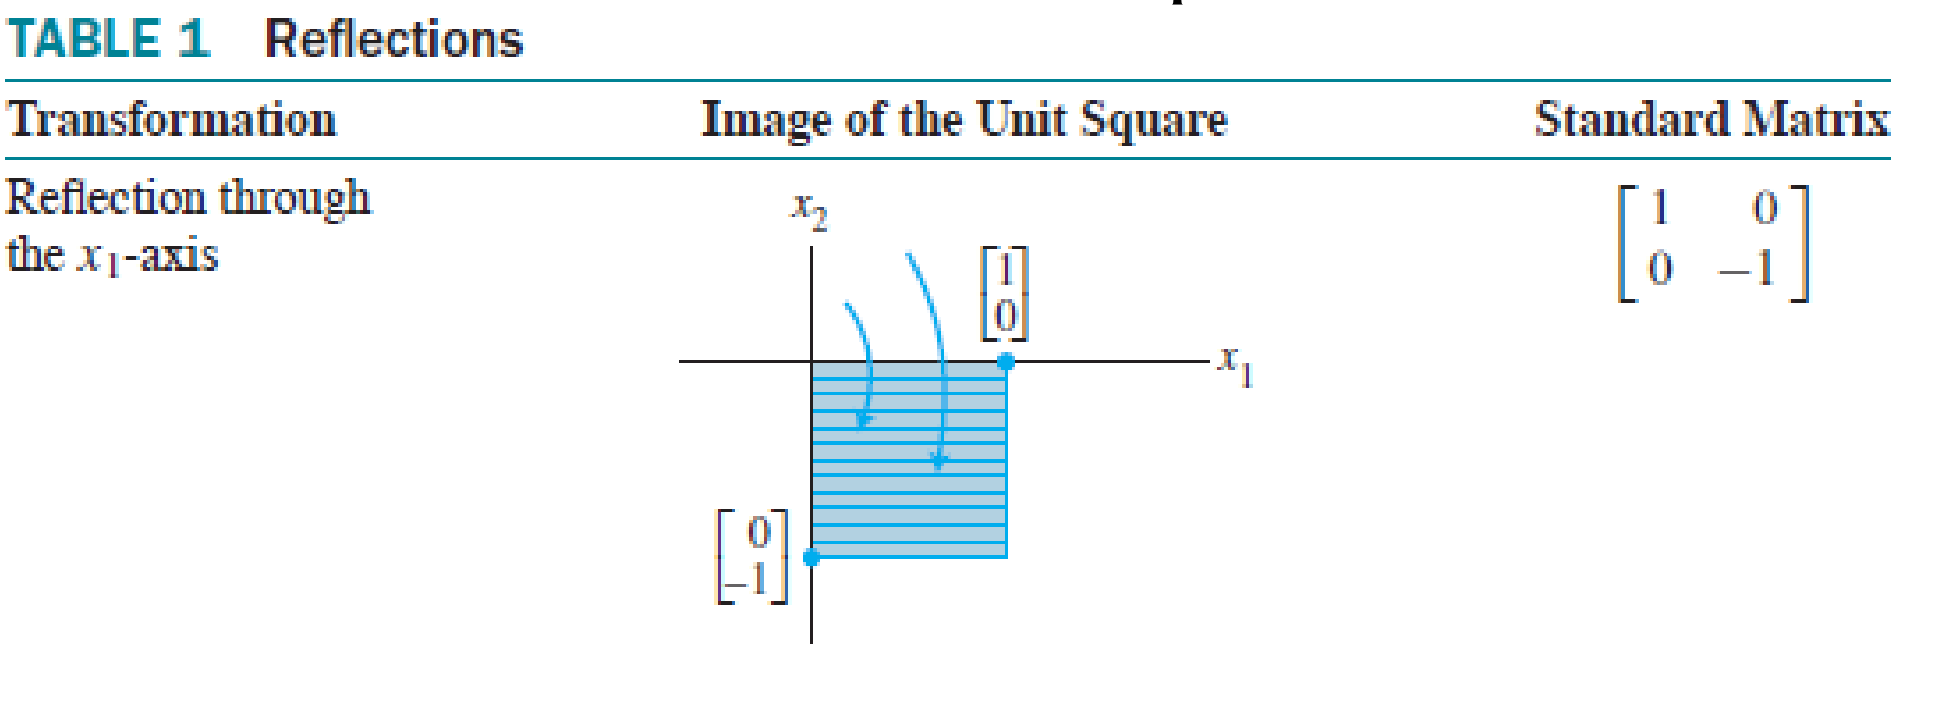
\includegraphics[width=.8\linewidth]{table1.png}
\end{figure}
\sourcepage{104}
\end{frame}

% Reference page 42
\begin{frame}{Reflections: Table 1 Continued}
  \begin{figure}
  \centering
  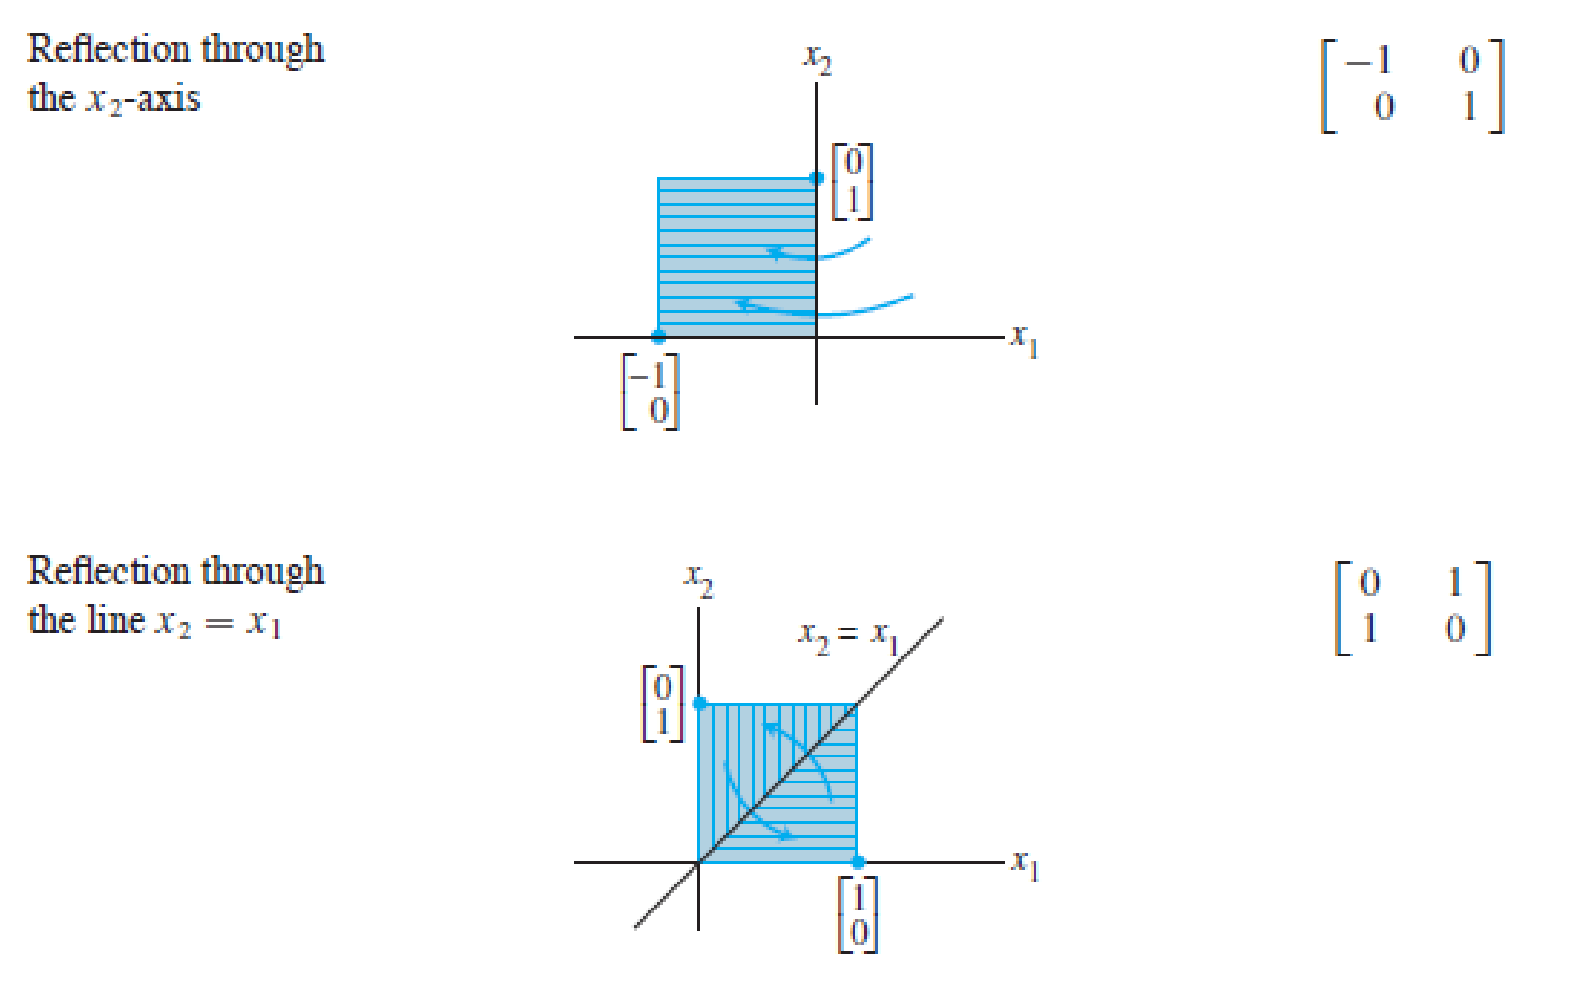
\includegraphics[height=.8\textheight]{table2.png}
\end{figure}
\sourcepage{105}
\end{frame}

% Reference page 43
\begin{frame}{Reflections: Table 1 Continued}
 \begin{figure}
  \centering
  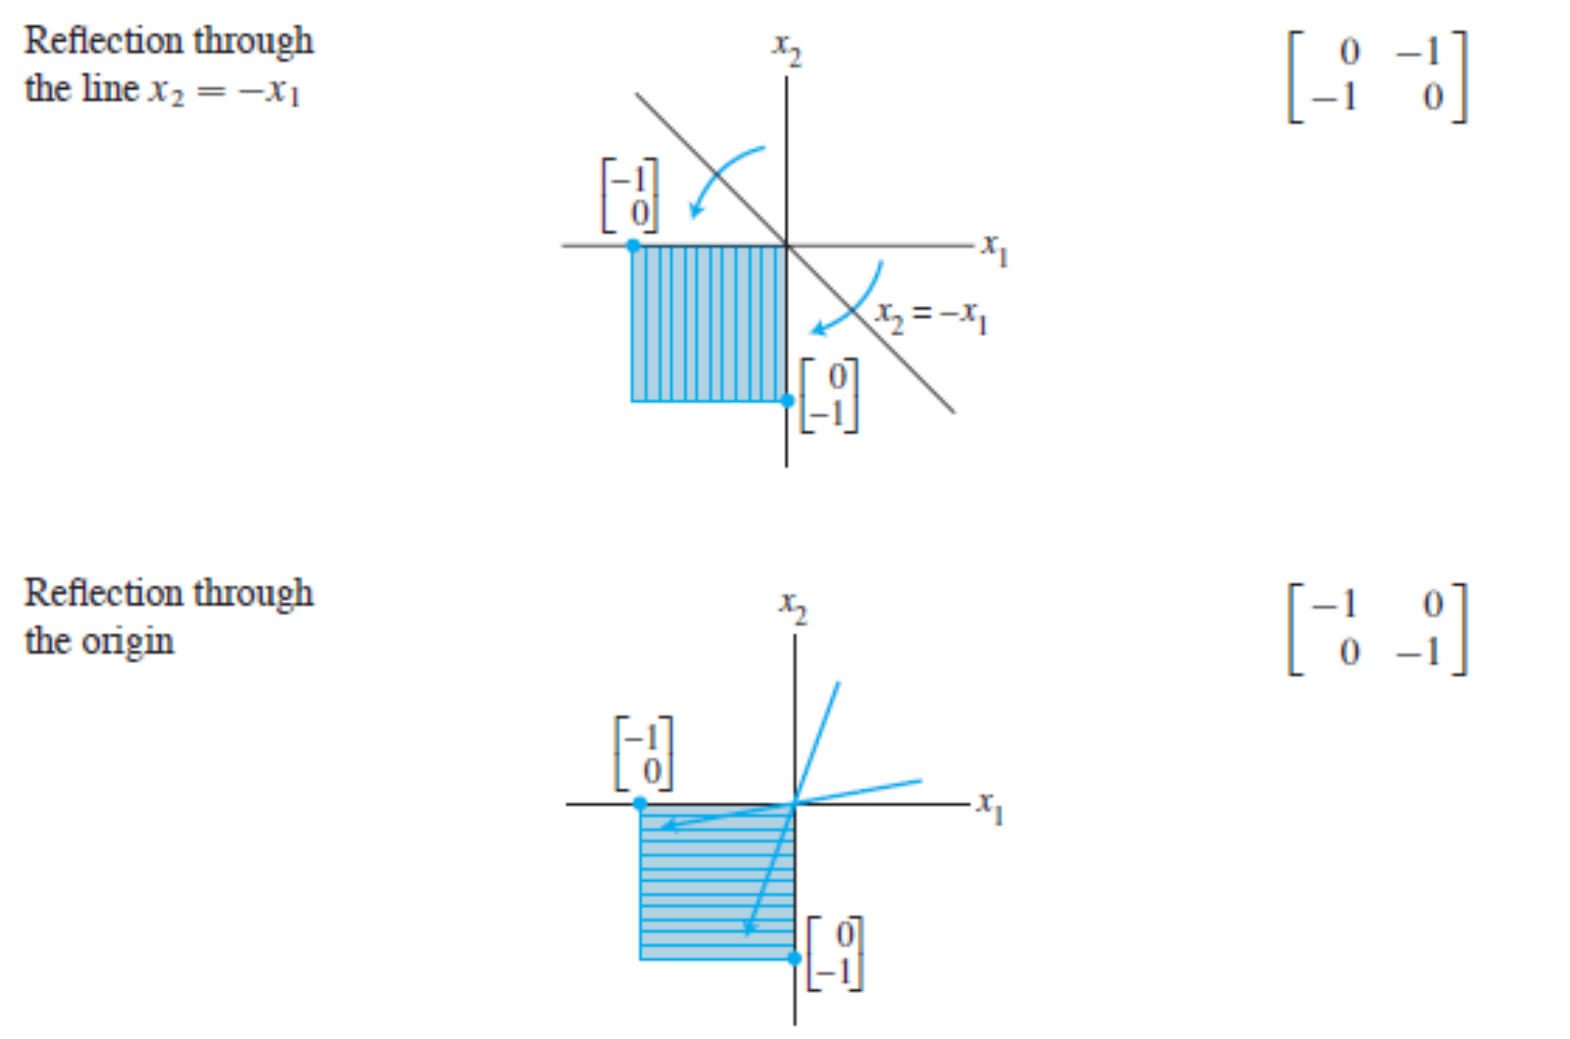
\includegraphics[height=.8\textheight]{table3.png}
\end{figure}
  \sourcepage{106}
\end{frame}

% Reference page 44


\begin{frame}{Table 2: Contractions and Expansions}
  \only<1>{
    \begin{columns}
        \begin{column}{.5\linewidth}
          \begin{figure}
            \centering
            
\includegraphics[width=\linewidth]{contraction3.png}
          \end{figure}
        \end{column}
        \begin{column}{.5\linewidth}
          \begin{figure}
            \centering
            
\includegraphics[width=\linewidth]{contraction4.png}
          \end{figure}
        \end{column}
      \end{columns}
  }
  \only<2>{
     \begin{columns}
    \begin{column}{.5\linewidth}
      \begin{figure}
        \centering
        
\includegraphics[width=\linewidth]{expansion1.png}
      \end{figure}
    \end{column}
    \begin{column}{.5\linewidth}
      \begin{figure}
        \centering
        
\includegraphics[width=\linewidth]{expansion2.png}
      \end{figure}
    \end{column}
  \end{columns}
  }
\end{frame}
\begin{frame}[shrink=10]{Table 2: Contractions and Expansions}
 \begin{figure}
  \centering
  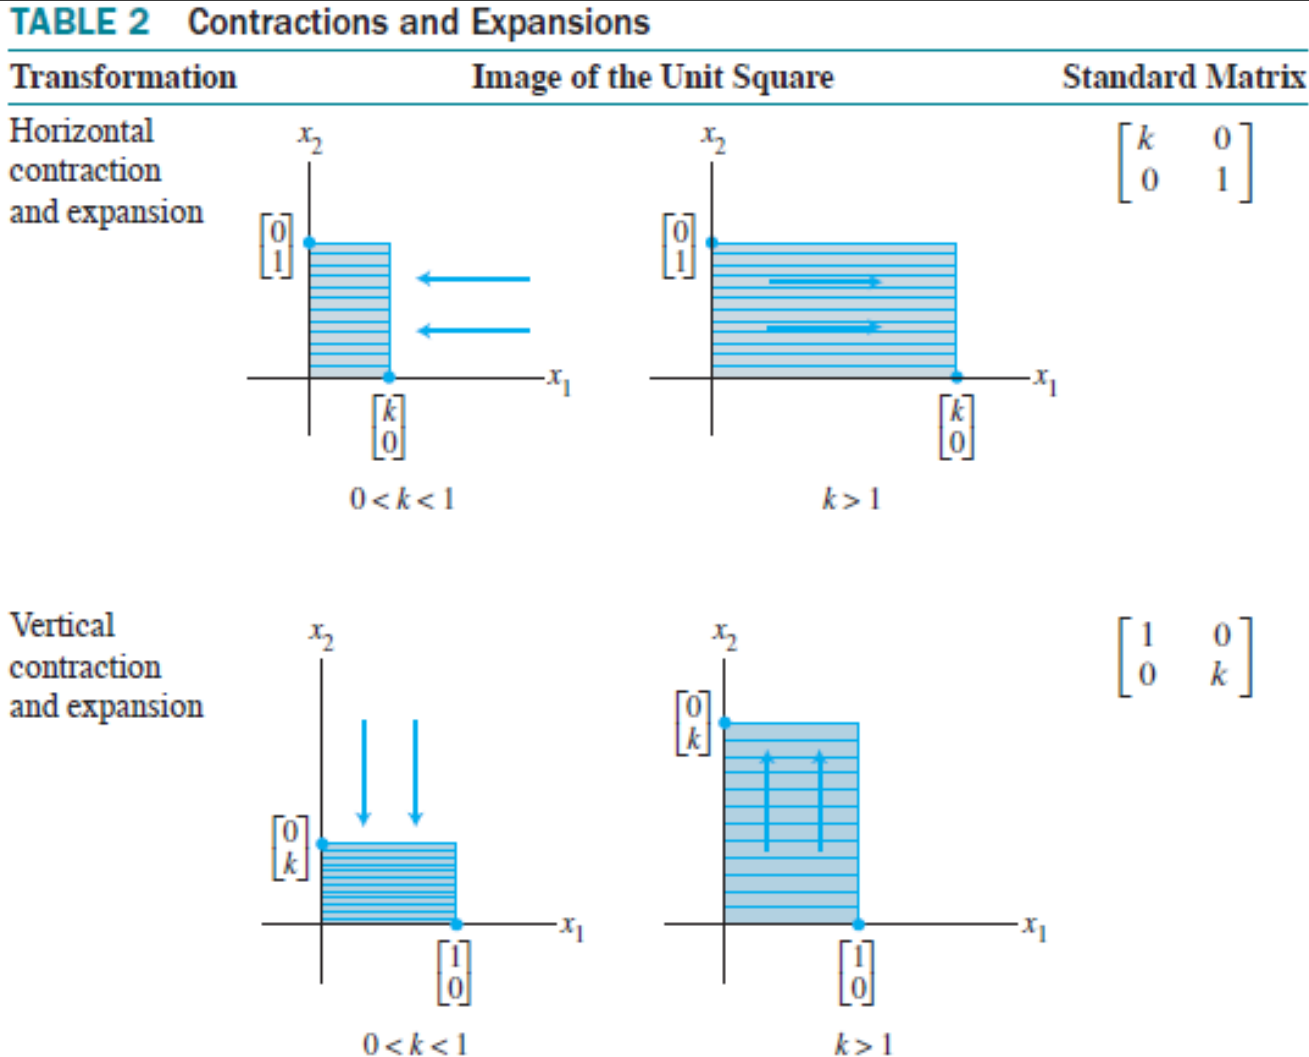
\includegraphics[height=\textheight]{table4.png}
\end{figure}
\sourcepage{107}
\end{frame}



\begin{frame}{Table 3: Shears}
  \begin{columns}
    \begin{column}{.5\linewidth}
      \begin{figure}
        \centering
        
\includegraphics[width=\linewidth]{sheer1.png}
      \end{figure}
    \end{column}
    \begin{column}{.5\linewidth}
      \begin{figure}
        \centering
        
\includegraphics[width=\linewidth]{sheer2.png}
      \end{figure}
    \end{column}
  \end{columns}
\end{frame}
% Reference page 45
\begin{frame}[shrink=10]{Table 3: Shears}
 \begin{figure}
  \centering
  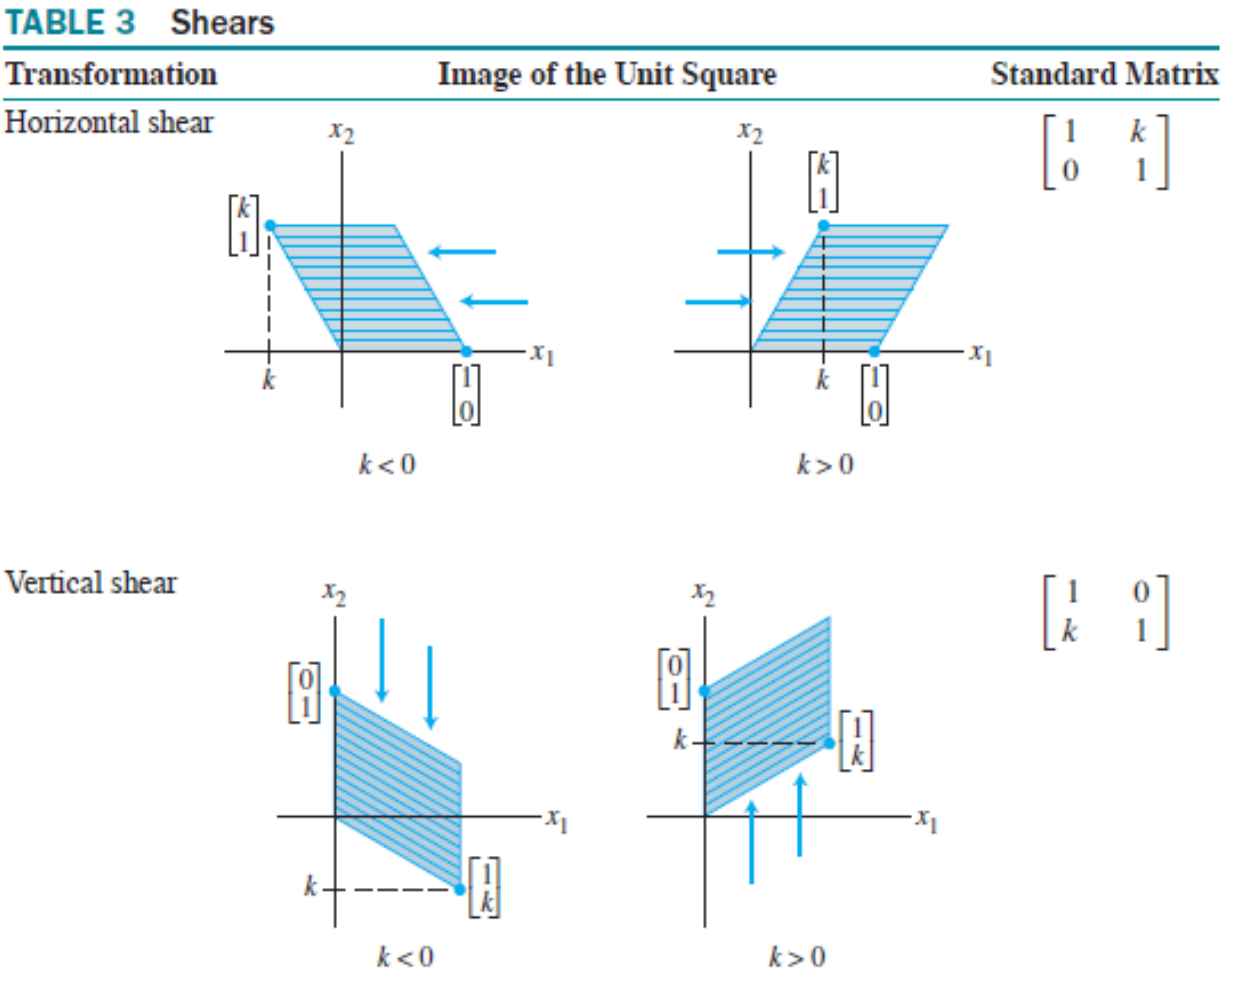
\includegraphics[height=\textheight]{table5.png}
\end{figure}
\sourcepage{108}
\end{frame}

\begin{frame}{Table 4: Projections}
  \begin{columns}
    \begin{column}{.5\linewidth}
      \begin{figure}
        \centering
        
\includegraphics[width=\linewidth]{projection1.png}
      \end{figure}
    \end{column}
    \begin{column}{.5\linewidth}
      \begin{figure}
        \centering
        
\includegraphics[width=\linewidth]{projection2.png}
      \end{figure}
    \end{column}
  \end{columns}
\end{frame}
% Reference page 46
\begin{frame}{Table 4: Projections}
   \begin{figure}
  \centering
  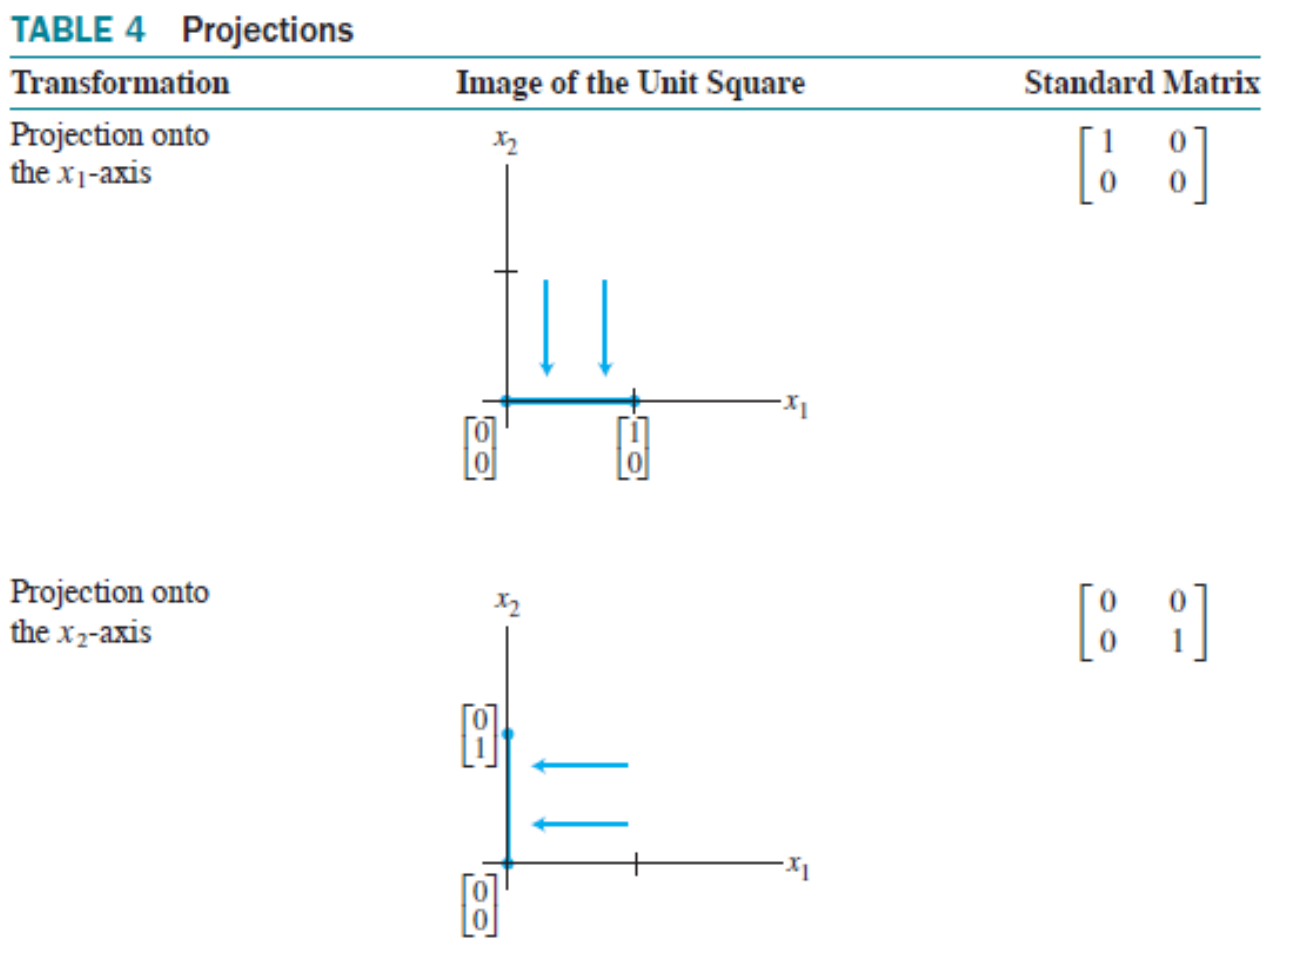
\includegraphics[height=.8\textheight]{table6.png}
\end{figure}
  
  \sourcepage{109}
\end{frame}

% Reference page 47
\section[Existence]{Existence and Uniqueness Questions}
\begin{frame}{Existence and Uniqueness Questions}
\begin{block}{Definition}
A mapping $T:\R^n\to\R^m$ is said to be \textbf{onto} $\R^m$ if each
$\vect b\in\R^m$ is the image of at least one $\vect x\in\R^n$.
\end{block}

\begin{itemize}
  \item Equivalently, $T$ is onto $\mathbb{R}^m$ when the range of $T$ is all of the codomain $\mathbb{R}^m$. 
  \item That is, $T$ maps $\mathbb{R}^n$ onto $\mathbb{R}^m$ if, for each $\vect b$ in the codomain $\mathbb{R}^m$, there exists at least one solution of T(x)=b. 
  \item "Does T map $\mathbb{R}^n$ onto $\mathbb{R}^m$?" is an existence question.
  \item The mapping $T$ is not onto $\mathbb{R}^m$ when there is some $\vect b$ in $\mathbb{R}^m$ for which the equation T(x)=b has no solution. See the figure on the next slide. 
\end{itemize}
% for every $\vect b\in\R^m$, the equation
% \[
% T(\vect x)=\vect b
% \]
% has at least one solution. This is an existence question. The mapping is not
% onto when some $\vect b$ makes the equation inconsistent.
\sourcepage{110}
\end{frame}

% Reference page 48
\begin{frame}{Onto and One-to-One}
\begin{columns}[T]
\column{.48\textwidth}
\centering
\begin{tikzpicture}[>=Stealth,scale=.65]
\fill[blue!15] (-2,-1.2)--(-.5,-.8)--(-.5,1.2)--(-2,1.6)--cycle;
\draw[->,lectureblue] (-.2,.4)--(1,.4) node[midway,above]{$T$};
\fill[blue!18] (1.3,-1)--(2.7,-.7)--(2.7,1.1)--(1.3,1.4)--cycle;
\node at (2,-1.35){Range $=\R^m$};
\end{tikzpicture}

\scriptsize $T$ is onto $\R^m$.
\column{.48\textwidth}
\centering
\begin{tikzpicture}[>=Stealth,scale=.65]
\fill[blue!15] (-2,-1.2)--(-.5,-.8)--(-.5,1.2)--(-2,1.6)--cycle;
\draw[->,lectureblue] (-.2,.4)--(1,.4) node[midway,above]{$T$};
\fill[blue!18] (1.3,-.35)--(2.7,-.1)--(2.7,.65)--(1.3,.9)--cycle;
\node at (2,-1.35){Range $\subsetneq\R^m$};
\end{tikzpicture}

\scriptsize $T$ is not onto $\R^m$.
\end{columns}
\medskip
\begin{block}{Definition of One-to-one}
A mapping $T:\R^n\to\R^m$ is said to be \textbf{one-to-one} if every
$\vect b\in\R^m$ is the image of \textit{at most one} $\vect x\in\R^n$.
\end{block}
\sourcepage{111}
\end{frame}

% Reference page 49
\begin{frame}{Example 4: Onto and One-to-One}
Let $T$ be the linear transformation whose standard matrix is
\[
A=\begin{bmatrix}
1&-4&8&1\\
0&2&-1&3\\
0&0&0&5
\end{bmatrix}.
\]
Does $T$ map $\R^4$ onto $\R^3$? Is $T$ a one-to-one mapping?
\sourcepage{112}
\end{frame}

% Reference page 50
\begin{frame}{Example 4: Solution}
\textbf{Solution}:
\begin{itemize}
  \item Since $A$ is in echelon form, we can see at once that $A$ has a pivot position in each row.
  \item By Theorem 4 in Section 1.4, for each $\vect b$ in $\mathbb{R}^3$, the equation Ax=b is consistent. 
  \item In other words, the linear transformation T maps $\mathbb{R}^4$ (its domain) onto $\mathbb{R}^3$.
\end{itemize}

\medskip
However, since $A\vect x=\vect b$ has a {\color{red}{free variable}} because there are four
variables and only three basic variables, each $\vect b$ is the image of more than one $\vect x$. Thus $T$ is not one-to-one.
\sourcepage{113}
\end{frame}


\begin{frame}{Example 4: recap}
\begin{itemize}
  \item Check the echelon form of linear transformation:
  \item If consistent: maps domain to codomain.
  \item If and only if no free variable: one-to-one mapping
\end{itemize}
\sourcepage{113}
\end{frame}

\begin{frame}{Kernel and Range of a Linear Transformation}
Some vectors may be mapped to $\vect 0$.

\begin{figure}
  \centering
  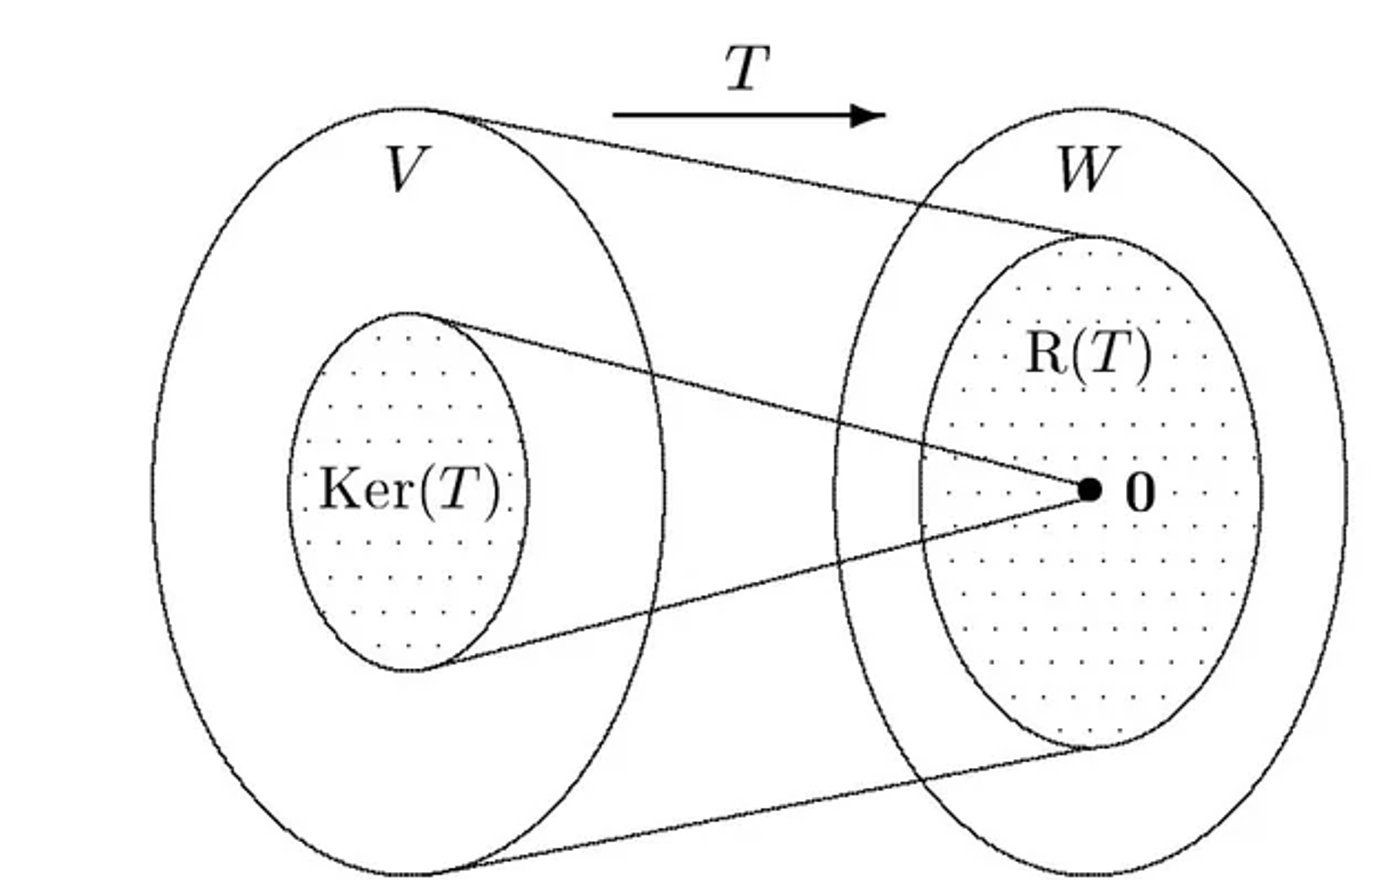
\includegraphics[width=.5\linewidth]{kernel.png}
\end{figure}
\end{frame}

\begin{frame}{How to understand these...}
\only<1>{
  \begin{figure}
  \centering
  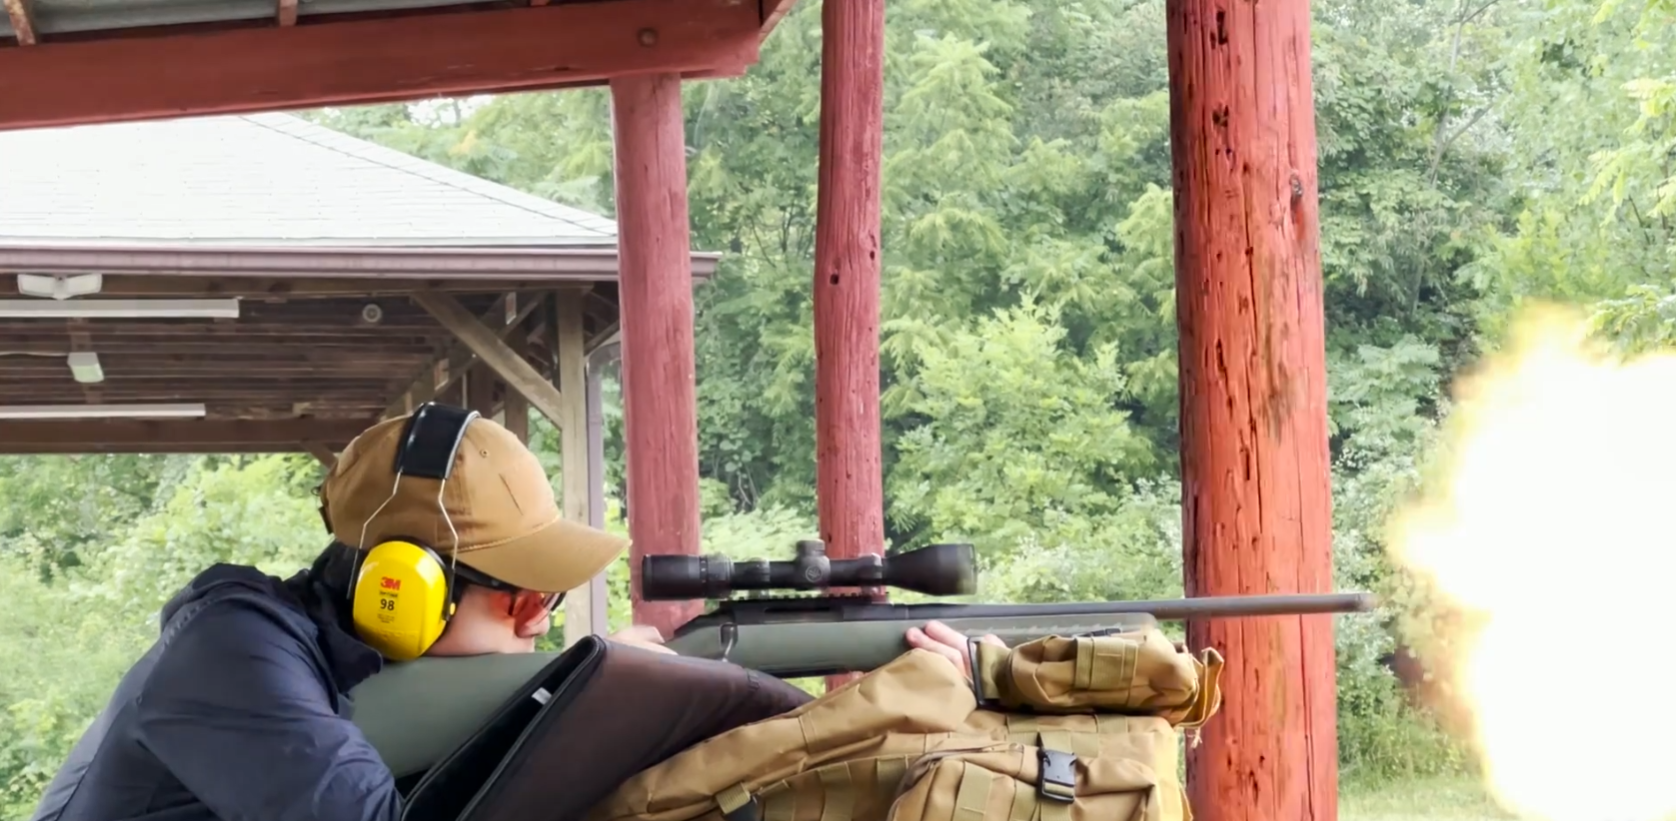
\includegraphics[width=.8\linewidth]{rifle.png}
  \end{figure}
}
\only<2>{
  \begin{figure}
  \centering
  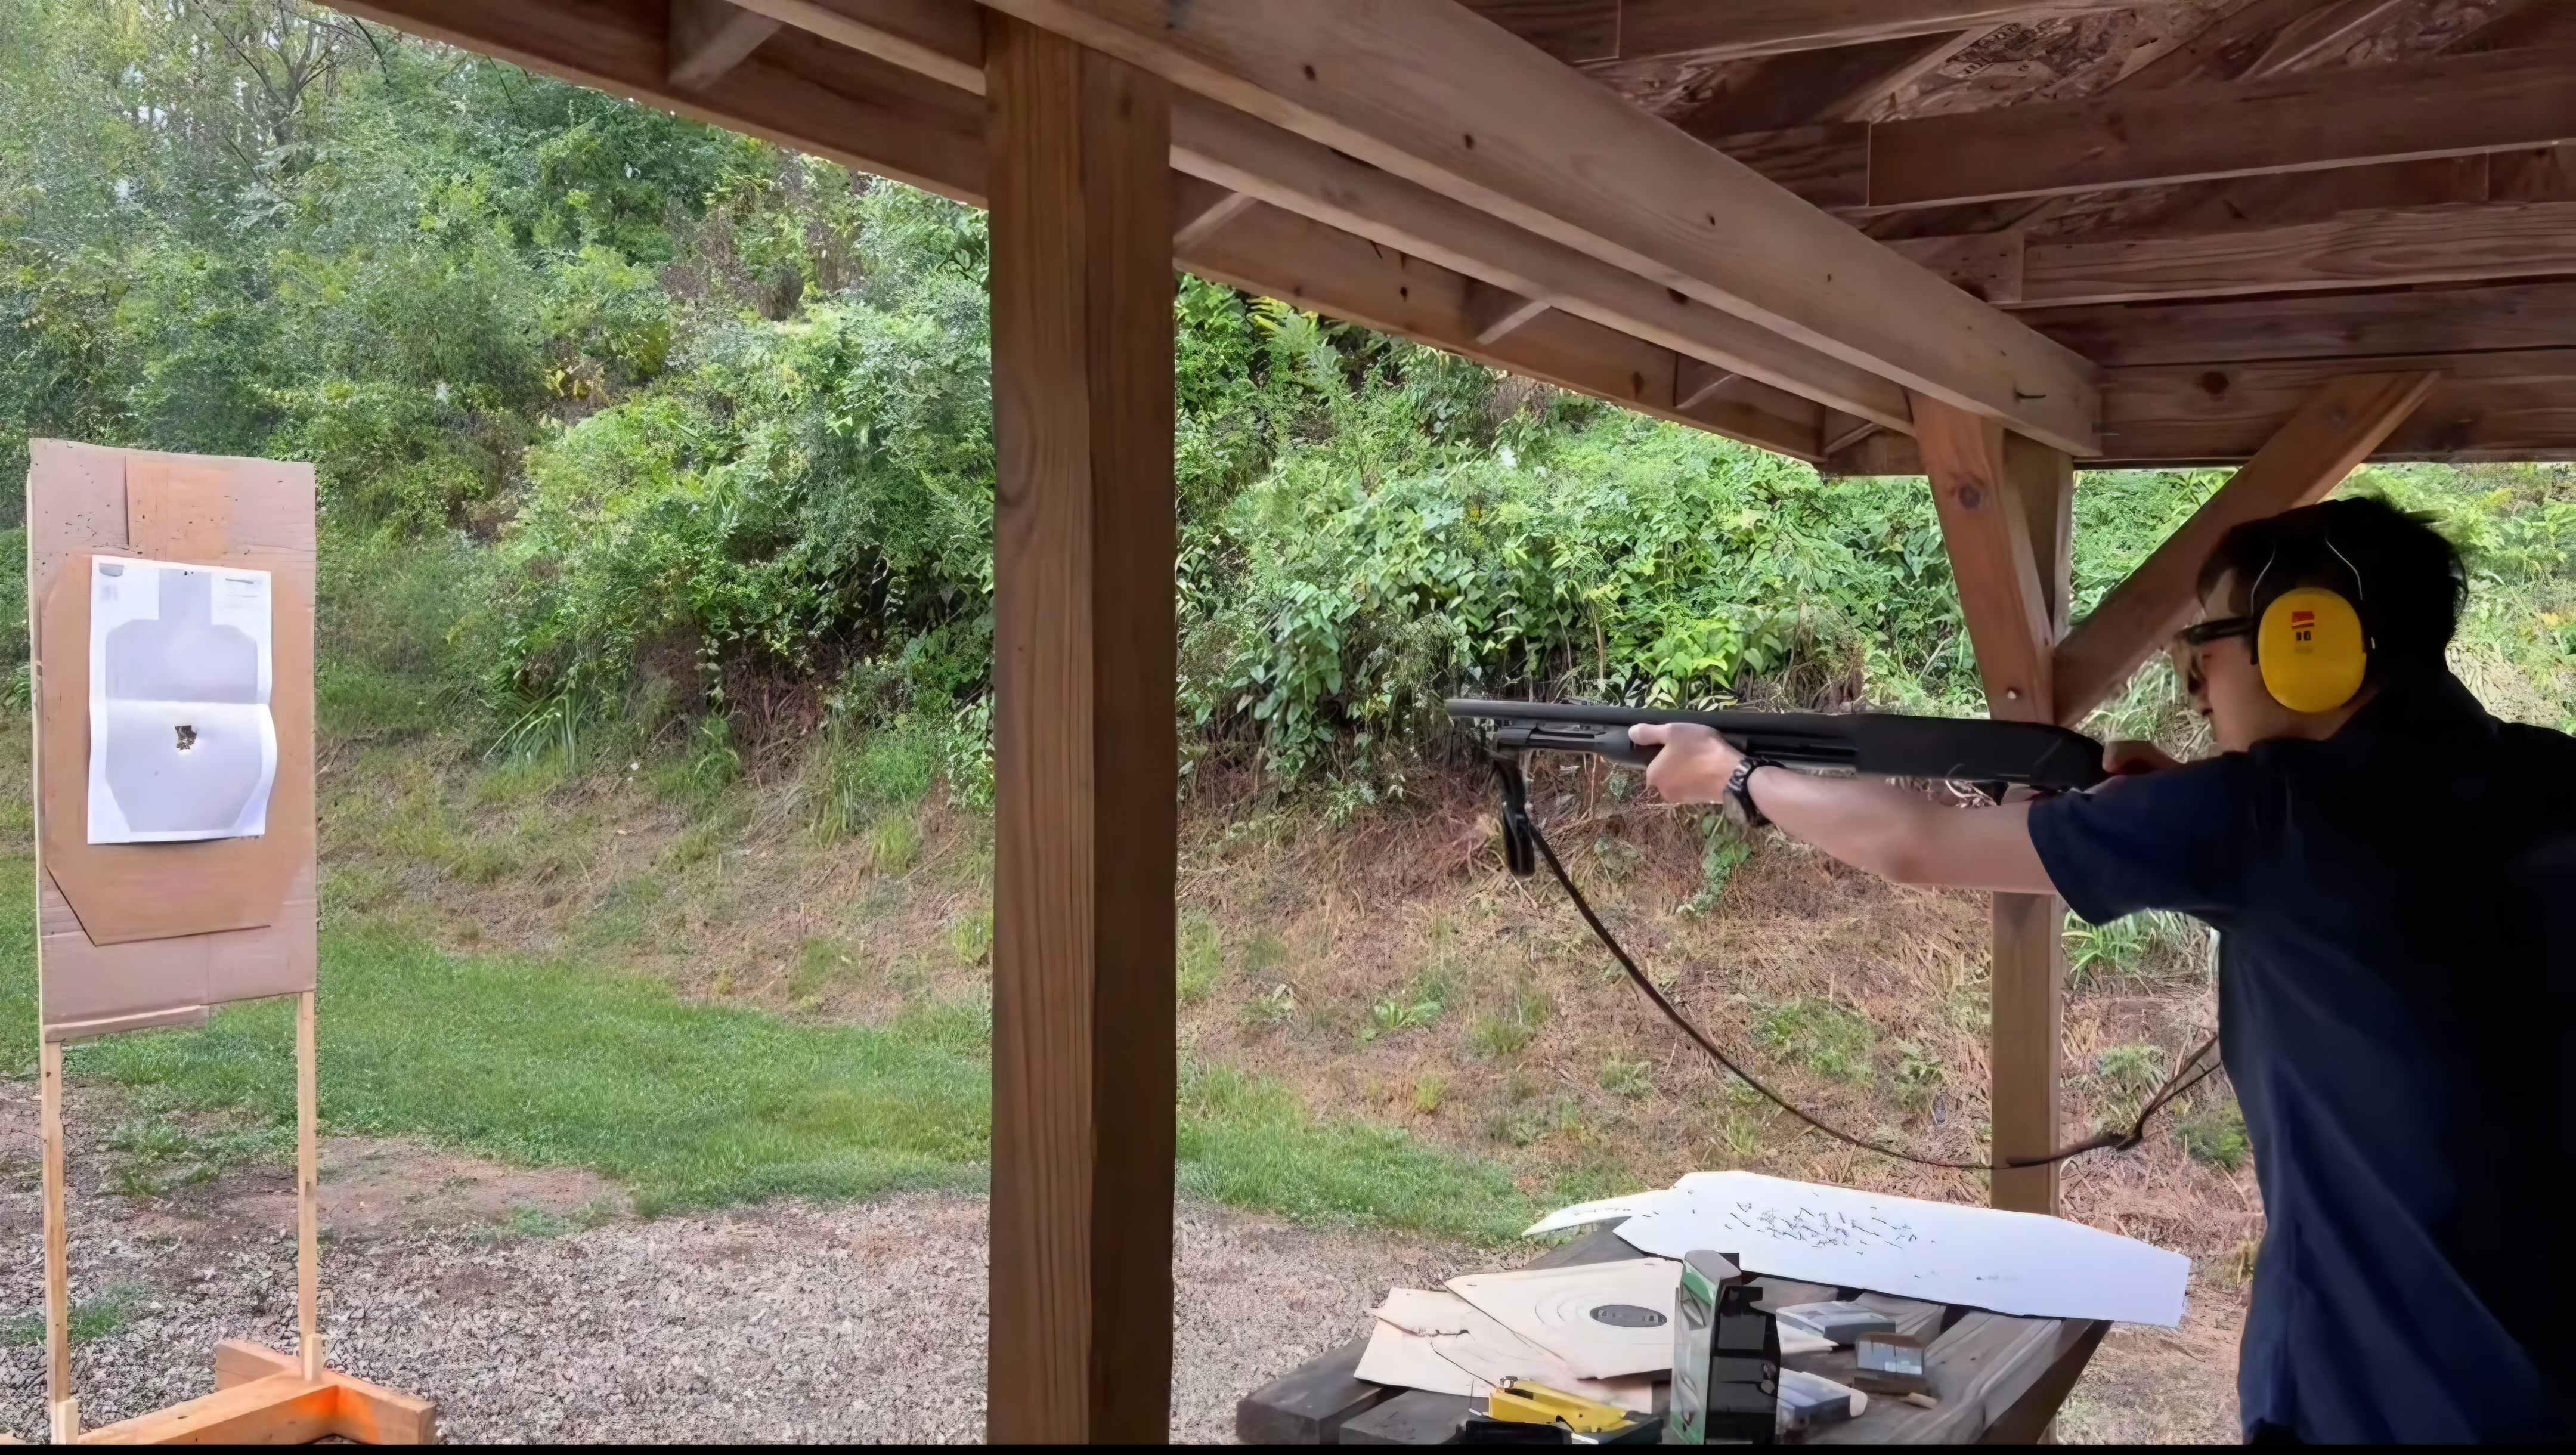
\includegraphics[width=.8\linewidth]{shotgun.jpg}
  \end{figure}
}
\only<3>{
  \begin{figure}
  \centering
  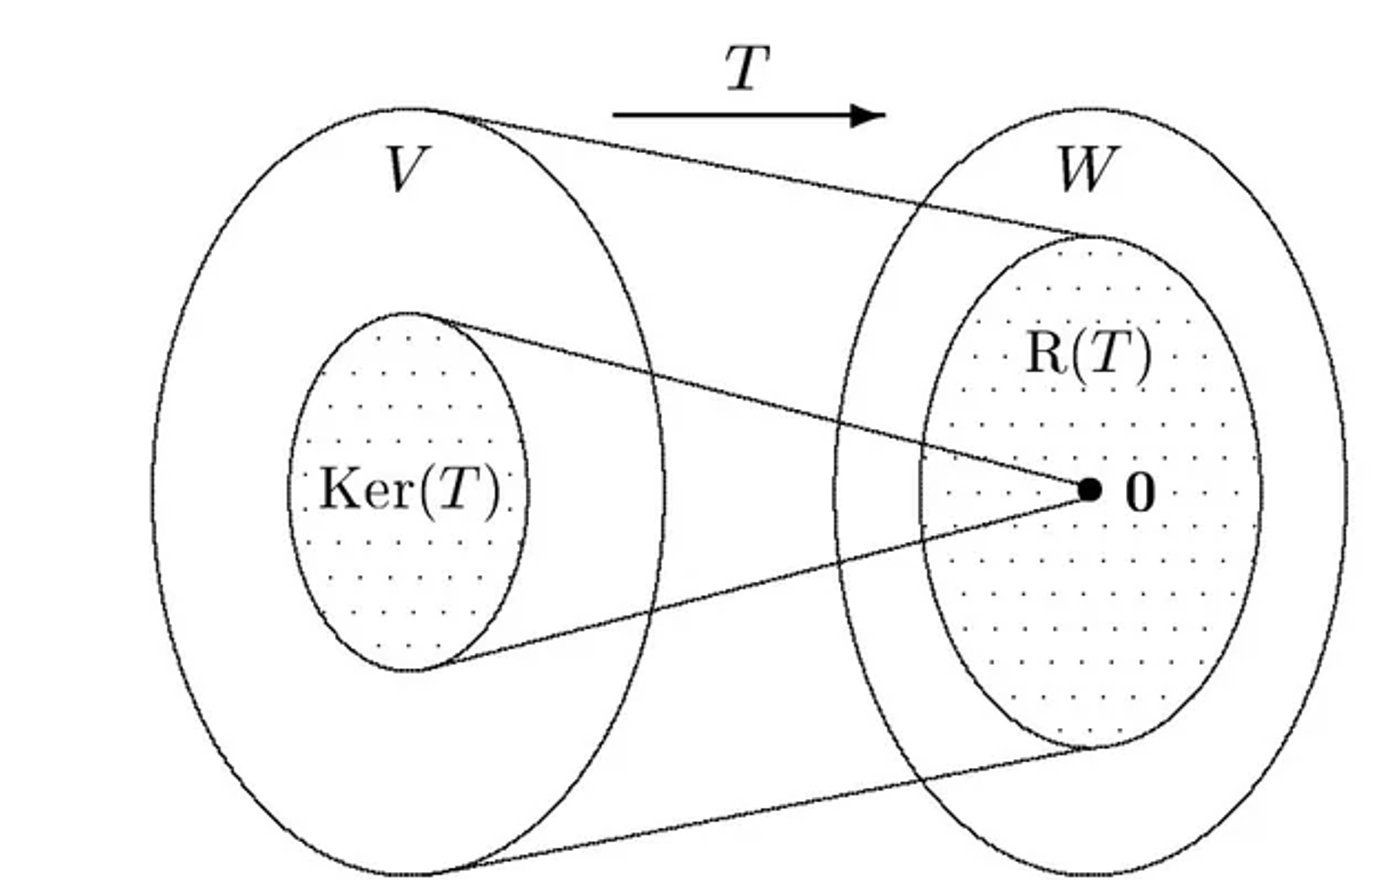
\includegraphics[width=.5\linewidth]{kernel.png}
  \end{figure}
  
}
\end{frame}

% Reference page 51
\begin{frame}{Kernel and Range of a Linear Transformation}
Subspaces of vector spaces other than $\R^n$ are often described in terms of a linear transformations instead of matrices.
\begin{block}{Definition}
A {\color{lectureblue}\textbf{linear transformation} $T$} from a vector space $V$ into a vector space $W$ is a rule that assigns to each $\vect x\in V$ a unique vector $T(\vect x)\in W$, such that
\begin{enumerate}
\item $T(\vect u+\vect v)=T(\vect u)+T(\vect v)$ for all $\vect u,\vect v\in V$;
\item $T(c\vect u)=cT(\vect u)$ for every $\vect u\in V$ and scalar $c$.
\end{enumerate}
\end{block}
The \textbf{kernel} is $\{\vect x\in V:T(\vect x)=\vect0\}$; the
\textbf{range} is $\{T(\vect x):\vect x\in V\}$.
\sourcepage{114}
\end{frame}

% Reference page 52
% \begin{frame}{Glossary}
% \renewcommand{\arraystretch}{1.15}
% \begin{tabular}{r>{\bfseries}l>{\bfseries}l}
% 1.&Square matrix&方阵\\
% 2.&(Row) Column Vector&(行)列向量\\
% 3.&Parallelogram rule&平行四边形法则\\
% 4.&Scalar multiplication&数乘\\
% 5.&Linear combination&线性组合\\
% 6.&Parametric vector form&参数向量形式\\
% 7.&(Non)Homogeneous&(非)齐次的\\
% 8.&(Non)Trivial solution&(非)平凡解\\
% \end{tabular}
% \sourcepage{115}
% \end{frame}
